\documentclass[a4paper, 12pt]{article}

\usepackage{geometry}
\usepackage{amsmath}
\usepackage{gvv}

\title{Question 2.10.29}
\author{AI25BTECH11040 - Vivaan Parashar}
\date{\today}

\begin{document}

\maketitle

\section{Question: }
The volume of the parallelopiped whose sides are given by $\textit{a} = 2\vec{i}-2\vec{j}$, $\textit{b} = \vec{i}+\vec{j}-\vec{k}$, $\textit{OC} = 3\vec{i} - \vec{k}$, is

\section{Solution: }
Let's define the position vectors $\vec{a}$, $\vec{b}$ and $\vec{c}$ as follows:
\begin{align}
    \vec{a} = \myvec{2      \\ -2 \\ 0}, \quad
    \vec{b} = \myvec{1      \\ 1 \\ -1}, \quad
    \vec{c} = \myvec{3      \\ 0 \\ -1}\\
\end{align}
To find the volume of the parallelopiped, we use the scalar triple product formula:

\begin{align}
    V = |\det(\myvec{\vec{a}\, \vec{b}\, \vec{c}})|\text{, where }\\
    \therefore V = \left|\det\left(\myvec{2 & 1 & 3 \\ -2 & 1 & 0 \\ 0 & -1 & -1}\right)\right|\\
    \therefore V = 2
\end{align}

\section{Plot: }
\begin{figure}[h!]
    \centering
    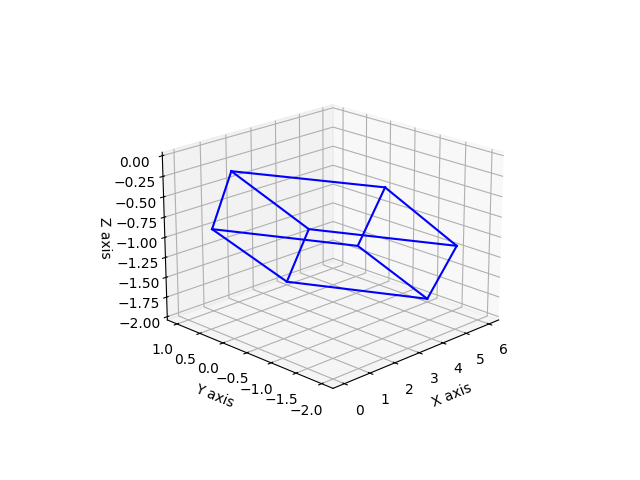
\includegraphics[width=\columnwidth]{figs/plot.png}
    \caption{Parallelopiped formed by vectors $\vec{a}$, $\vec{b}$ and $\vec{c}$}
    \label{fig:2.10.29}
\end{figure}


\end{document}